% ====================================================================
% SUPERSEDED. This draft is written against the SYNTHETIC testbed, in which
% the ESG -> distress relationship is INJECTED by the generator at gamma=-4.0.
% Every number in it is from generated data and none of them describe the real
% Bloomberg panel.
%
% The current paper is paper/cresta_real.tex, generated from the pipeline's
% own artefacts by src/generate_paper.py. See paper/README.md.
%
% Kept as the record of the earlier work. Do not cite results from this file.
% ====================================================================
%% CRESTA — IEEE conference version (condensed to ~8 pages)
%% Compile from the esg_distress_project/ directory so that
%% reports/figures/*.png resolve:  pdflatex cresta_ieee.tex  (run twice)
%% Requires: IEEEtran.cls, graphicx, amsmath, amssymb, booktabs

\documentclass[conference]{IEEEtran}
\IEEEoverridecommandlockouts

\usepackage{cite}
\usepackage{amsmath,amssymb,amsfonts}
\usepackage{graphicx}
\usepackage{booktabs}
\usepackage{array}
\usepackage{textcomp}
\usepackage{xcolor}
\usepackage[hidelinks]{hyperref}

\newcommand{\code}[1]{\texttt{\small #1}}

\begin{document}

\title{Beyond Circularity: A Forward-Looking Evaluation\\
Framework for ESG-Augmented Corporate\\
Distress Prediction}

\author{\IEEEauthorblockN{Anonymous Author(s)}
\IEEEauthorblockA{Submission under double-blind review}}

\maketitle

\begin{abstract}
Contemporary corporate distress models frequently report ROC-AUC scores above
0.95. We argue that a large fraction of that performance is an artifact.
Where the distress label is derived from accounting quantities that also appear
among the predictors, the classifier is not asked to forecast anything; it only
has to reconstruct the identity used to build the label. We refer to this
condition as label circularity, and treat it as a form of target leakage that is
specific to distress modelling. CRESTA is an evaluation framework designed around
two constraints: a one-year separation between the feature vector $X_t$ and the
label $Y_{t+1}$, and the removal of any feature that is circular with respect to
the distress definition. To check that the framework can still recover a real
effect after those constraints are applied, we constructed a synthetic panel of
60{,}000 firms observed over ten fiscal years (2015--2024), with a known ESG
influence ($\gamma = -4.0$) embedded in the distress-generating process. On a
strictly out-of-time test set of 115{,}873 firm-years containing 264 distress
events (prevalence 0.2278\%), a financial-only model (Model~A) reached ROC-AUC
0.5348, and the addition of four ESG features (Model~B) raised this to 0.6117. A
2{,}000-iteration percentile bootstrap gave a mean difference of $+0.0774$ (95\%
CI $[+0.0455,\, +0.1080]$), and SHAP attribution placed the three ESG variables
first, second, and third. These findings establish controlled signal recovery
under non-circular conditions. They do not speak to real-market performance;
testing on India's mandated BRSR disclosures is left for later work.
\end{abstract}

\begin{IEEEkeywords}
Corporate distress prediction, label circularity, target leakage, ESG
integration, gradient boosting, out-of-time validation, SHAP, class imbalance
\end{IEEEkeywords}

\section{Introduction}

Firms fail, and the people who lend to them, hold their paper, or regulate them
would like as much warning as possible. Predicting corporate financial
distress, meaning a firm's inability to meet its obligations before default or
restructuring actually occurs, is one of the older quantitative problems in
finance. The methods have changed a great deal over the decades. Altman's
Z-score \cite{altman1968} gave way to logistic regression \cite{ohlson1980},
then to structural models built on option-pricing ideas \cite{merton1974}, and
more recently to gradient-boosted tree ensembles \cite{chen2016,ke2017}. Reported
discrimination has climbed with each step, and it is now common to see ROC-AUC
figures north of 0.95.

We think many of those figures should be read with suspicion. Suppose a study
defines distress from a small set of accounting variables, for example negative
book equity, or interest coverage below one, and then hands the model those same
accounting variables (or ratios computed from them) as inputs. There is no
forecasting problem left to solve. The model can post a near-perfect score by
learning the arithmetic that produced its own target. A classifier that reaches
0.99 ROC-AUC because it has noticed that current liabilities exceed current
assets has told us nothing about the coming year; it has read the balance sheet
that is already in front of it and sorted on that. This is the pattern we call
label circularity. It is close kin to target leakage \cite{sculley2015}, though
the two are not identical: leakage usually means future information contaminating
the training set, whereas circularity is contemporaneous, with label and
features drawn from one and the same accounting period. Both fail the same way in
the end. Sculley and colleagues \cite{sculley2015} catalogue how such
dependencies accumulate unnoticed in deployed systems, and Rabanser et al.
\cite{rabanser2019} show that a strong holdout number is a poor guarantee once
the input distribution moves.

A second issue sits on top of this one, and it is why the paper is framed around
ESG. Regulators are now producing standardised non-financial disclosure in
volume; India's BRSR mandate is one example. Sustainable-finance research has
long suggested that ESG measures carry information about slow-moving risks,
governance failures, regulatory exposure, transition risk, that a current
balance sheet has not yet absorbed \cite{friede2015}. That is a testable claim.
But it cannot be tested cleanly on a pipeline that is still contaminated by
circularity, because a handful of circular financial features will dominate the
fit and leave nothing for a marginal ESG signal to explain.

So the questions run together. Very little published work checks whether a
reported distress result holds up once temporal separation, circular-feature
removal, and out-of-time evaluation are all imposed at once, and fewer studies
still do that while looking for a known orthogonal signal in the same pass. That
combination is what CRESTA is built to test. The framework enforces a strict
one-year lag between features and labels; it flags and drops features that are
circular with the distress definition; and it supplies a controlled setting in
which an ESG signal of known size is injected and then either recovered or not.
None of the individual pieces are novel. What we offer is the assembly, the
synthetic validation, and a fairly detailed account of what happened.

Three questions organise the study. RQ1 asks how apparent performance changes
when the circular features are taken out. RQ2 asks whether a known ESG signal can
be pulled back out of a non-circular, forward-looking pipeline. RQ3 asks how
class imbalance and the choice of decision threshold should change the way any of
these numbers are read, given how rare distress actually is in the panel.

Our contributions are the framework itself, which isolates circularity and
measures the discrimination lost when it is removed; a synthetic-data result
showing statistically significant recovery of a planted ESG signal after that
removal, with $\Delta$AUC $= +0.0774$ and a 95\% interval of $[+0.0455,\,
+0.1080]$; a threshold analysis at 0.2278\% prevalence, where we show that a
model can advertise 98\%-plus accuracy while catching under two percent of real
distress events; and SHAP evidence that Model~B leans on the ESG features about
as heavily as the injected mechanism implies it should.

\section{Related Work}

\textbf{Classical and machine-learning distress prediction.}
Altman's five-ratio discriminant model \cite{altman1968}, fitted on
manufacturing firms in the 1960s, is still a working reference in credit
practice. Ohlson \cite{ohlson1980} moved the problem onto logistic regression;
the Black--Scholes--Merton tradition \cite{merton1974} took a different route,
treating equity as an option and reading off a distance-to-default from asset
volatility and leverage. All of these are transparent but restrictive: linear or
log-linear structure, a handful of fixed inputs \cite{jones2015}. Tree ensembles
loosened those restrictions. XGBoost \cite{chen2016} and LightGBM \cite{ke2017}
now routinely top classical baselines on tabular credit data, both in
credit-scoring surveys \cite{lessmann2015} and in bankruptcy-specific
comparisons \cite{barboza2017}, with support vector machines close behind
\cite{bellotti2009}. The added flexibility is a double-edged thing. It makes
circularity more dangerous, not less, because a high-capacity model asked to
predict a target that is a deterministic function of its own inputs will simply
fit that function. Note that this is not the usual temporal-leakage story, where
tomorrow's data leaks into today's training fold. Circularity is same-period:
one accounting statement, used twice. Sculley et al. \cite{sculley2015} describe
how these hidden couplings pile up in production ML, and Rabanser et al.
\cite{rabanser2019} give evidence that impressive holdout accuracy tends to hide
distribution-shift fragility.

\textbf{ESG and default risk.}
Friede, Busch and Bassen \cite{friede2015} pooled more than two thousand
empirical studies and found a mostly positive ESG--performance association,
which has kept institutional interest high \cite{bassen2006}. The underlying
evidence is not tidy, though. Effect sizes swing by sector, by region, and by
which ESG pillar is measured, and nobody has settled the direction of
causation. Any attempt to show that ESG data adds a distress signal beyond
financials has to first get the circular financial features out of the way,
which is precisely what most existing models do not do.

\textbf{Validity and explainability.}
The argument for strict out-of-time testing in credit modelling is old and
well supported \cite{jones2015,lessmann2015}. SHAP \cite{lundberg2017} gives
per-prediction feature attributions grounded in cooperative game theory; in this
paper it does one narrow job, which is to confirm that Model~B's ESG features are
carrying their own weight rather than proxying for size or profitability. The
gap we see, and the one CRESTA is meant to fill, is that almost no distress study
verifies its performance, or a candidate ESG signal, against all three of
temporal separation, circular-feature removal, and out-of-time evaluation at
once, in a setting where the true answer is known in advance.

\section{The CRESTA Framework}

\subsection{Pipeline and synthetic panel}
The pipeline is a fixed sequence: generate the synthetic data, run it through the
quality gates, engineer features, ablate the circular ones, build the temporally
shifted target, split out of time, train, evaluate, and finally run the post-hoc
explainers. Figure~\ref{fig:arch} lays it out.

\begin{figure*}[t]
\centering
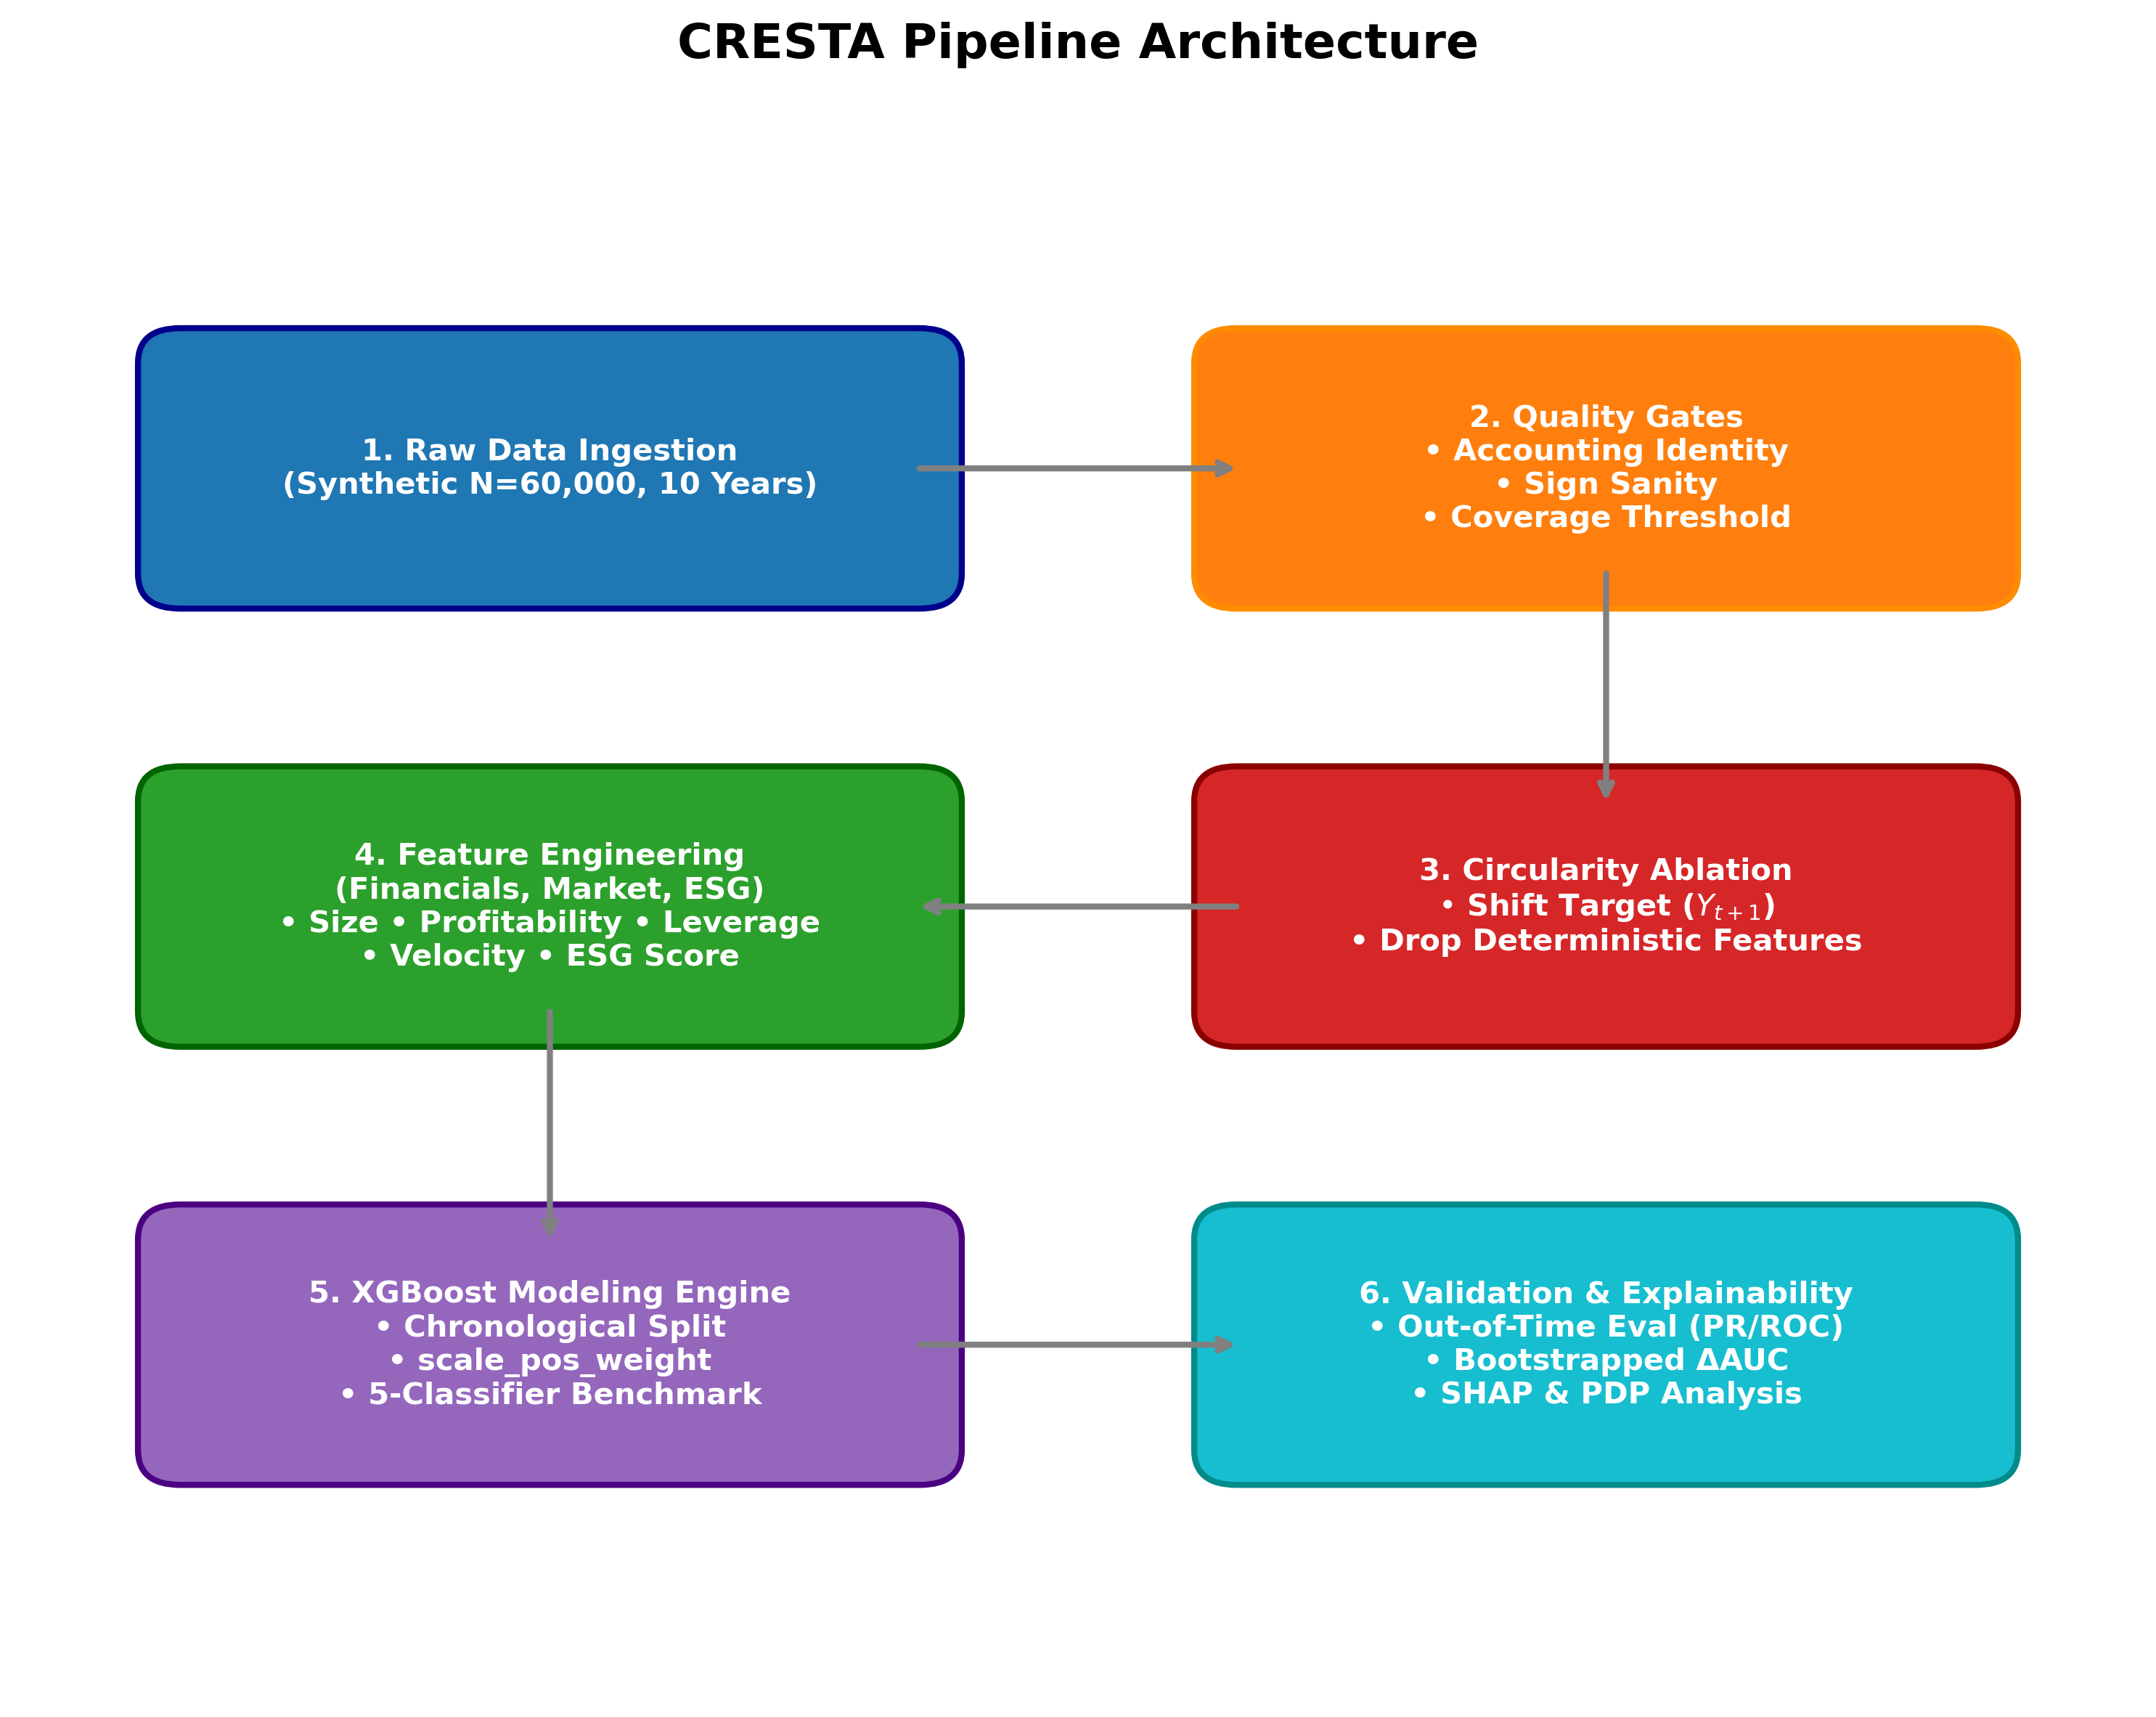
\includegraphics[width=0.9\textwidth]{reports/figures/cresta_architecture.png}
\caption{The CRESTA pipeline. Synthetic generation feeds quality gating, feature
engineering, circular-feature ablation, temporal target construction, out-of-time
splitting, model training, and evaluation with post-hoc explainability.}
\label{fig:arch}
\end{figure*}

The panel holds $N = 60{,}000$ firms over $T = 10$ fiscal years (2015--2024),
generated under a fixed seed of 42, and it exists so that we know the ground
truth going in. Each firm is placed in one of 11 GICS sectors with a plausible
market weighting. Three latent drivers set its starting position: initial
log-total-assets from $\mathcal{N}(12.0,\,1.5)$, a base return on assets from
$\mathcal{N}(0.08,\,0.04)$, and an initial debt-to-total-capital ratio from
$\mathcal{N}(0.6,\,0.3)$. Then the firm evolves. Market capitalisation follows a
Geometric Brownian Motion,
\begin{equation}
dM_{i,t} = \mu_i\, M_{i,t}\, dt + \sigma_i\, M_{i,t}\, dW_{i,t},
\end{equation}
with drift $\mu_i = 0.05$ and volatility $\sigma_i = 0.1$. Profitability follows
an AR(1) process with an innovation standard deviation of 0.02, which reproduces
the mean reversion that real corporate earnings display:
\begin{equation}
\mathrm{ROA}_{i,t} = c + \phi\, \mathrm{ROA}_{i,t-1} + \epsilon_{i,t},
\qquad \epsilon_{i,t} \sim \mathcal{N}(0,\, \sigma_\epsilon^2).
\end{equation}
Survivorship is handled directly. If firm $i$ enters distress in year $t$, it
leaves the panel for every year after $t+1$, the way a real delisted name would.
Two sanity checks were run on the finished panel. A kernel-density comparison
showed the distressed firms sitting on a visibly left-shifted ROA distribution,
as intended. Separately, a correlation inspection confirmed that the financial
ratios carry the collinearities we wanted them to (ROA with EBIT margin, and so
on) while the ESG scores stay uncorrelated with profitability and leverage.

\subsection{The injected ESG signal}
Whether firm $i$ experiences distress in a given year is decided by a logistic
map from its latent state to a probability:
\begin{equation}
z_i = -2.0\, \mathrm{profit}_i + 0.5\, \mathrm{leverage}_i
      + \gamma\, \frac{\mathrm{base\_esg}_i}{100},
\qquad
p_i = \frac{1}{1 + e^{-(z_i - 2.0)}}.
\end{equation}
Here $\gamma = -4.0$ is the planted ESG effect, and a distress event fires when a
uniform draw comes in below $p_i$. Dividing by 100 puts the per-unit ESG
coefficient at $-4.0/100 = -0.04$, so, all else equal, a firm with a higher
latent ESG score has lower log-odds of distress by construction.

The model never sees \code{base\_esg} itself. It sees a noisy reading,
$\mathrm{e\_score}_i = \mathrm{clip}(\mathrm{base\_esg}_i + \epsilon_i,\, 0,\,
100)$ with $\epsilon_i \sim \mathcal{N}(0,\, 3)$; \code{s\_score} and
\code{g\_score} come from separate noise draws, and carbon intensity is a
size-scaled function of the environmental score. Since \code{e\_score} adds
noise of $\sigma = 3$ on top of a \code{base\_esg} whose standard deviation is
roughly 15, textbook measurement-error attenuation says a logistic regression on
the observed score should return a coefficient a little short of $-0.04$:
\begin{equation}
\hat{\beta} \approx -0.04 \times
\frac{\sigma_{\text{signal}}^2}{\sigma_{\text{signal}}^2 + \sigma_{\text{noise}}^2}
= -0.04 \times \frac{225}{234} \approx -0.0385.
\label{eq:coefmap}
\end{equation}
The five-stage diagnostic in Section~\ref{sec:diag} recovers roughly $-0.035$,
which is about where you would expect it to land once boundary clipping and the
linear approximation to a non-linear generator are accounted for. We treat this
as a theoretical target that the empirical estimate happens to hit, and not as
anything stronger.

\subsection{Quality gating}
All 594{,}392 raw firm-year rows pass through seven gates before any feature
engineering. In order: primary-key integrity, which blocks the whole batch on a
violation; the accounting identity $|\mathrm{TA}-(\mathrm{TL}+\mathrm{TE})| < 2\%$,
which only flags; sign sanity on total assets, which is the one hard-fail gate on
the row level and dropped 5{,}943 rows; a range check on ROA and interest
coverage, flag-only; a coverage gate requiring 70\% non-null across seven core
fields, which flagged 2{,}097 rows but left them in the training set rather than
removing them; a temporal-continuity gate that warns on gaps longer than two
years; and a scale check on $|Z''|$. What comes out is 588{,}449 rows, and
$594{,}392 - 5{,}943 = 588{,}449$ exactly.

\subsection{Features, ablation, and the temporal target}
Feature engineering yields 44 features, grouped by economic role: leverage and
solvency, liquidity, profitability, the classical composites (Altman $Z''$, the
EMS score, their diagnostic flags), temporal dynamics (year-on-year deltas,
multi-year trends, consecutive-loss and consecutive-low-coverage counters), size
and sector controls, and the four ESG features.

Six of the 44 are circular with the usual distress definitions and are removed
outright: \code{interest\_coverage} and its capped and below-1-flag variants,
\code{X4\_equity\_to\_liabilities}, \code{liabilities\_to\_assets}, and
\code{negative\_equity\_flag}. That leaves 38 features going into the model. The
three counts, 44 engineered, 6 removed, 38 used, are kept distinct throughout the
paper because they are easy to conflate.

The target is shifted forward by one fiscal year within each ticker,
$y_{i,t} = \mathrm{is\_distress\_event}_{i,\,t+1}$, which in code is a group-wise
\code{shift(-1)} on the firm identifier. After the shift, $X_{i,t}$ predicts
$Y_{i,t+1}$, so the task is a one-year-ahead forecast rather than a
same-year classification.

\subsection{Experimental setup}
The split is temporal and unshuffled: 2015--2022 for training (472{,}576 rows,
1{,}739 positives, prevalence 0.3680\%) and 2023--2024 for testing (115{,}873
rows, 264 positives, 0.2278\%). The training imbalance,
$470{,}837 / 1{,}739 = 270.75$, is used directly as XGBoost's
\code{scale\_pos\_weight}.

Five classifiers across four families were run: logistic regression with balanced
class weights, Gaussian naive Bayes, a depth-10 decision tree, a 200-tree random
forest at depth 15, and XGBoost with 200 trees, depth 4, learning rate 0.05,
0.8 subsample and column-sample, and \code{scale\_pos\_weight} $= 270.75$. No
hyperparameter was tuned against the test set, and there was no cross-validation
or grid search. That is a genuine weakness of the study, and the XGBoost
settings are probably not optimal. The upside is that model selection could not
have leaked anything from the test period, because model selection did not
happen.

For the ablation, two XGBoost models share the same hyperparameters and the same
split. Model~A uses 34 financial and market features with the ESG columns
dropped; Model~B uses all 38. Nothing else differs between them.

At 0.2278\% prevalence, plain accuracy is nearly worthless as a summary, because
a classifier that always says ``healthy'' scores 99.77\%. We report ROC-AUC as
the headline, PR-AUC by trapezoidal integration of the precision--recall curve,
positive-class precision, recall and F1, and balanced accuracy; accuracy appears
only for context. To decide whether the ROC-AUC gap between the two models is
real, we ran a percentile bootstrap: 2{,}000 resamples with replacement, seed
42, the statistic being $\Delta$AUC $=$ ROC-AUC(B) $-$ ROC-AUC(A), and the
interval taken from the 2.5th and 97.5th percentiles, resampling rows. One
caveat we state up front: the test set has 58{,}677 firms and 57{,}196 of them
appear twice (2023 and 2024), so row-level resampling probably gives a slightly
tighter interval than a firm-level cluster bootstrap would. The interval is far
enough from zero that this is unlikely to matter for the conclusion.

The explainers are post-hoc and play no part in model choice: SHAP TreeExplainer
\cite{lundberg2017} on 10{,}000 sampled test rows, using mean absolute value for
the global ranking, and a partial dependence plot for \code{e\_score} over
5{,}000 test rows on a 50-point grid.

\section{Results}

\subsection{Benchmark and ablation}
Table~\ref{tab:bench} pulls discrimination apart from raw accuracy in the
rare-event regime. Logistic regression gives the best discrimination, at ROC-AUC
0.6520 with 65.15\% recall. Naive Bayes has the highest positive-class precision
but only recalls 2.27\% of events. The decision tree recalls a middling 55.30\%
with poor separation overall. Random forest is the cautionary case: 99.58\%
accuracy, zero distress events detected, and a balanced accuracy of 49.91\%,
which is below chance. XGBoost is the natural vehicle for the ablation. Its
ROC-AUC of 0.6117 and 51.52\% recall come from \code{scale\_pos\_weight} pushing
it hard toward the minority class, and it pays for that with a large number of
false positives.

\begin{table}[t]
\caption{Five-classifier benchmark on the out-of-time test set (2023--2024).
115{,}873 observations, 264 distress events (prevalence 0.2278\%). ROC-AUC and
balanced accuracy are the primary metrics; raw accuracy is for context.}
\label{tab:bench}
\centering
\renewcommand{\arraystretch}{1.2}
\setlength{\tabcolsep}{4pt}
\begin{tabular}{lcccccc}
\toprule
Classifier & Bal.\ Acc. & ROC-AUC & Prec.\ (+) & Rec.\ (+) & F1 (+) & Acc. \\
\midrule
Logistic Regr.\ & 61.85\% & \textbf{0.6520} & 0.358\% & \textbf{65.15\%} & \textbf{0.0071} & 58.56\% \\
Naive Bayes     & 50.44\% & 0.6353 & \textbf{0.370\%} & 2.27\%  & 0.0064 & 98.38\% \\
Decision Tree   & 57.09\% & 0.5626 & 0.306\% & 55.30\% & 0.0061 & 58.87\% \\
Random Forest   & 49.91\% & 0.6001 & 0.000\% & 0.00\%  & 0.0000 & \textbf{99.58\%} \\
XGBoost         & 59.26\% & 0.6117 & 0.355\% & 51.52\% & \textbf{0.0071} & 66.97\% \\
\bottomrule
\end{tabular}
\end{table}

The ablation result is in Table~\ref{tab:ablation}. With the circular features
gone and no ESG data, Model~A manages ROC-AUC 0.5348. That is only just above a
coin toss, and it is a long way below the near-perfect numbers that circular
studies report, which is the point: once you stop letting the model read its own
label, the financial ratios on their own do not say much about the following
year. Model~B, with the four ESG features added back, gets to 0.6117. PR-AUC goes
from 0.0027 to 0.0034, against a random-classifier floor of 0.0023 (the
prevalence). In relative terms Model~A sits at $1.19\times$ the floor and
Model~B at $1.51\times$, a 26\% improvement. Figure~\ref{fig:curves} shows both
sets of curves.

\begin{table}[t]
\caption{Ablation on the out-of-time test set. The two XGBoost models are
identical except that Model~B also receives the four ESG features.}
\label{tab:ablation}
\centering
\renewcommand{\arraystretch}{1.2}
\begin{tabular}{lcccc}
\toprule
Model & ROC-AUC & PR-AUC & $\Delta$AUC & Sig.? \\
\midrule
Model A (Fin.\ only)   & 0.5348 & 0.0027 & --      & --  \\
Model B (Fin.\ + ESG)  & 0.6117 & 0.0034 & $+0.0774$ & Yes \\
\bottomrule
\end{tabular}
\end{table}

\begin{figure*}[t]
\centering
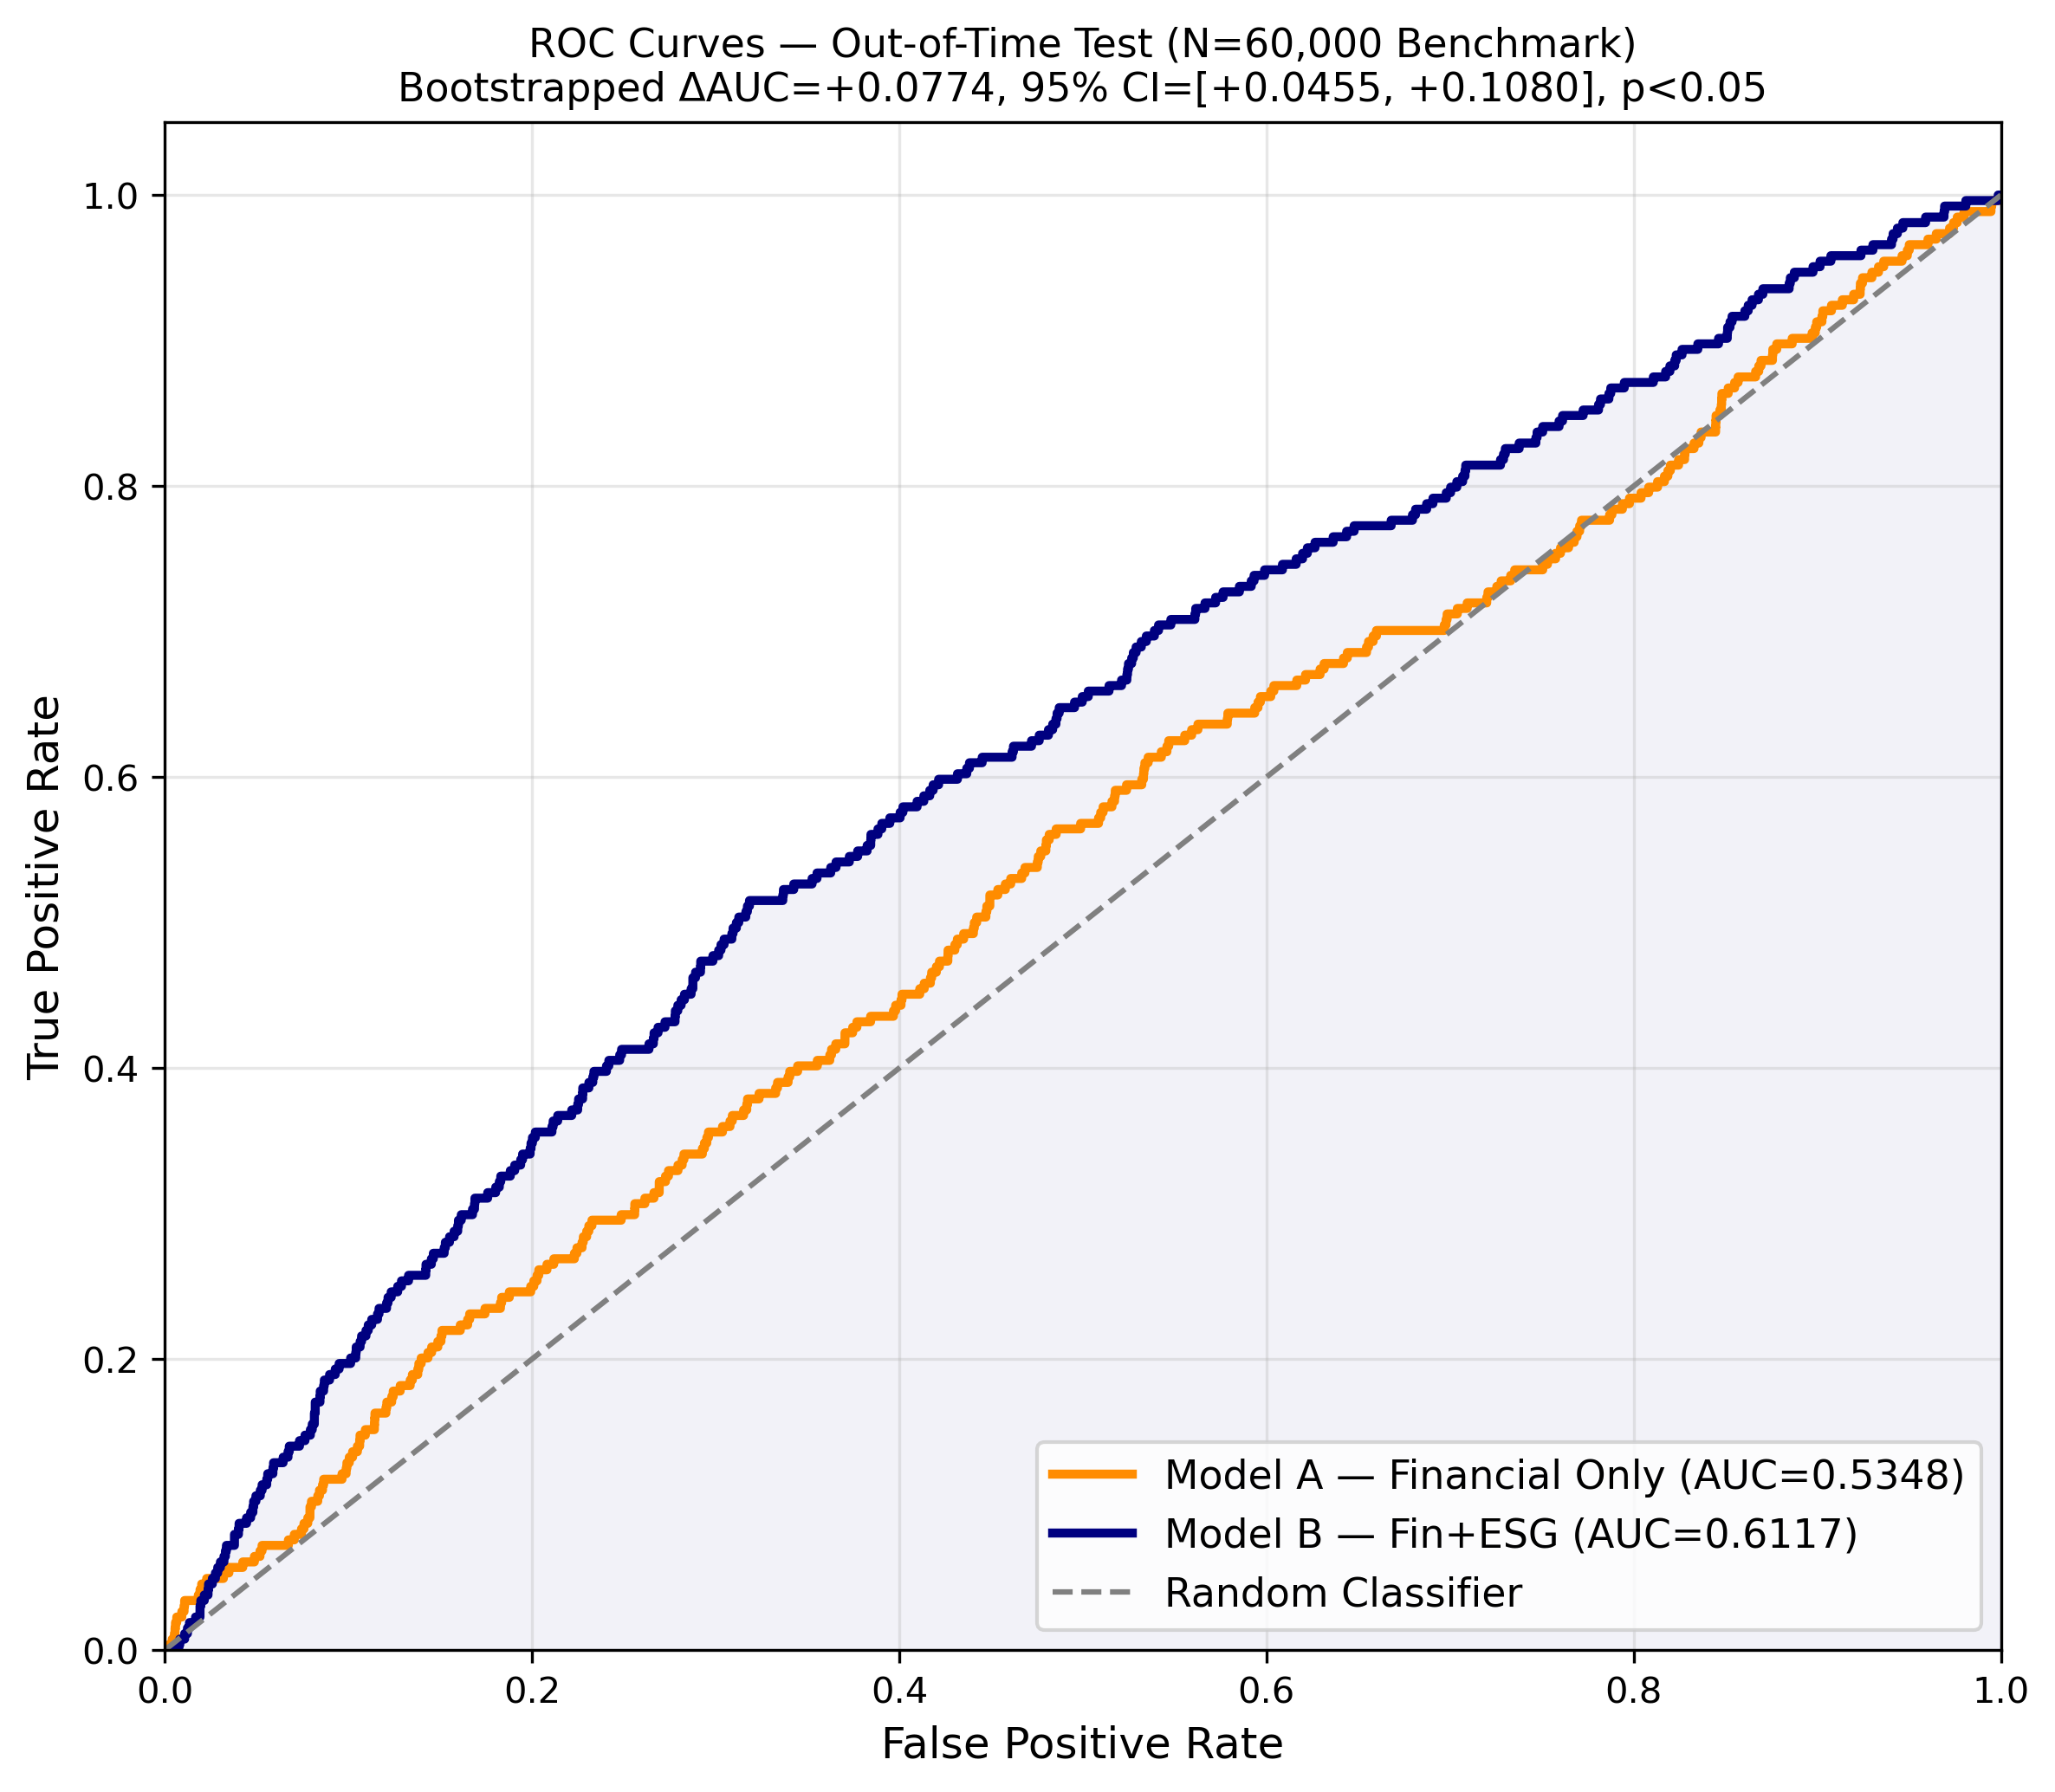
\includegraphics[width=0.47\textwidth]{reports/figures/roc_curve.png}
\hfill
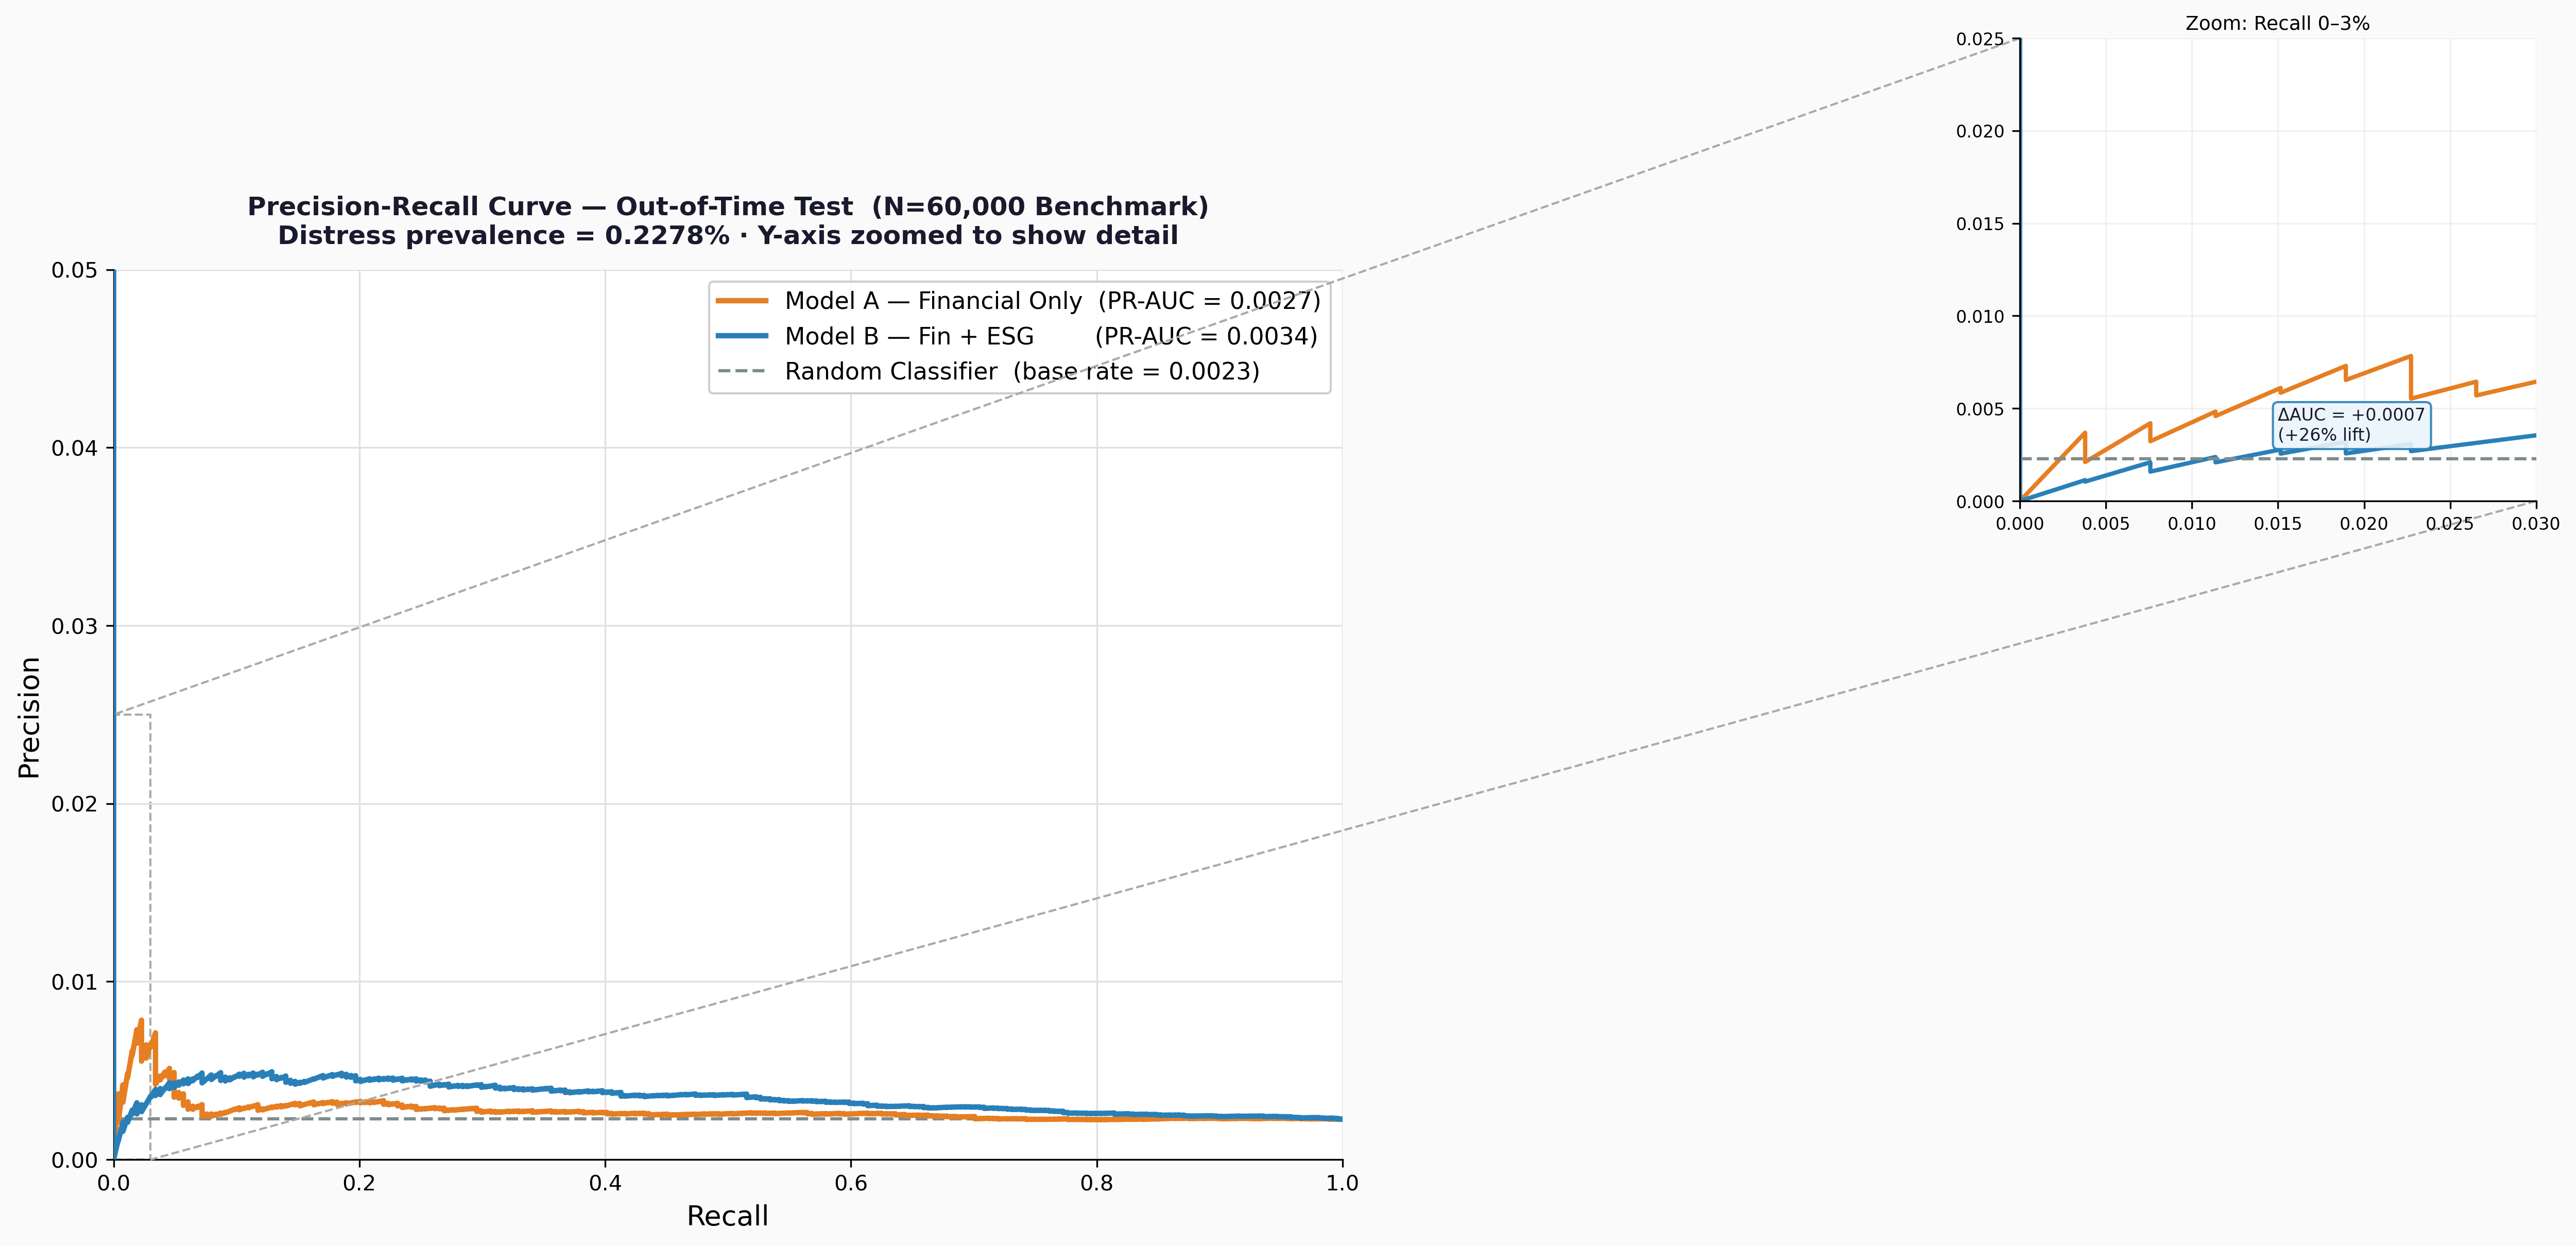
\includegraphics[width=0.47\textwidth]{reports/figures/pr_curve.png}
\caption{Left: ROC curves for Model~A (financial only, AUC $= 0.5348$) and
Model~B (financial $+$ ESG, AUC $= 0.6117$). The area between them is the
discrimination the ESG features add. Right: precision--recall curves, PR-AUC
0.0027 against 0.0034; the dashed line is the random-classifier floor
($= 0.0023$, the prevalence). Both models sit just above it.}
\label{fig:curves}
\end{figure*}

\subsection{Bootstrap significance}
The bootstrap (2{,}000 iterations, seed 42) returned a mean $\Delta$AUC of
$+0.0774$ with a 95\% interval of $[+0.0455,\, +0.1080]$. The interval is
entirely above zero, so the null that the two models perform the same is
rejected. A firm-level cluster bootstrap would give a wider interval, but the
lower bound is comfortably positive and we do not expect the sign of the
conclusion to change; a formal cluster version is on the future-work list.

\subsection{Operating characteristics and the threshold}
At the default 0.5 threshold, shown in Figure~\ref{fig:cm}, Model~B finds 136 of
264 events (51.52\% recall) and produces 38{,}148 false positives, for a
positive-class precision of 0.36\% and 66.97\% accuracy overall. The low
precision is arithmetic, not a broken model. When you are trying to find 264
needles among 115{,}609 non-needles, even a very small per-row false-positive
rate turns into tens of thousands of false alarms in absolute terms.

\begin{figure}[t]
\centering
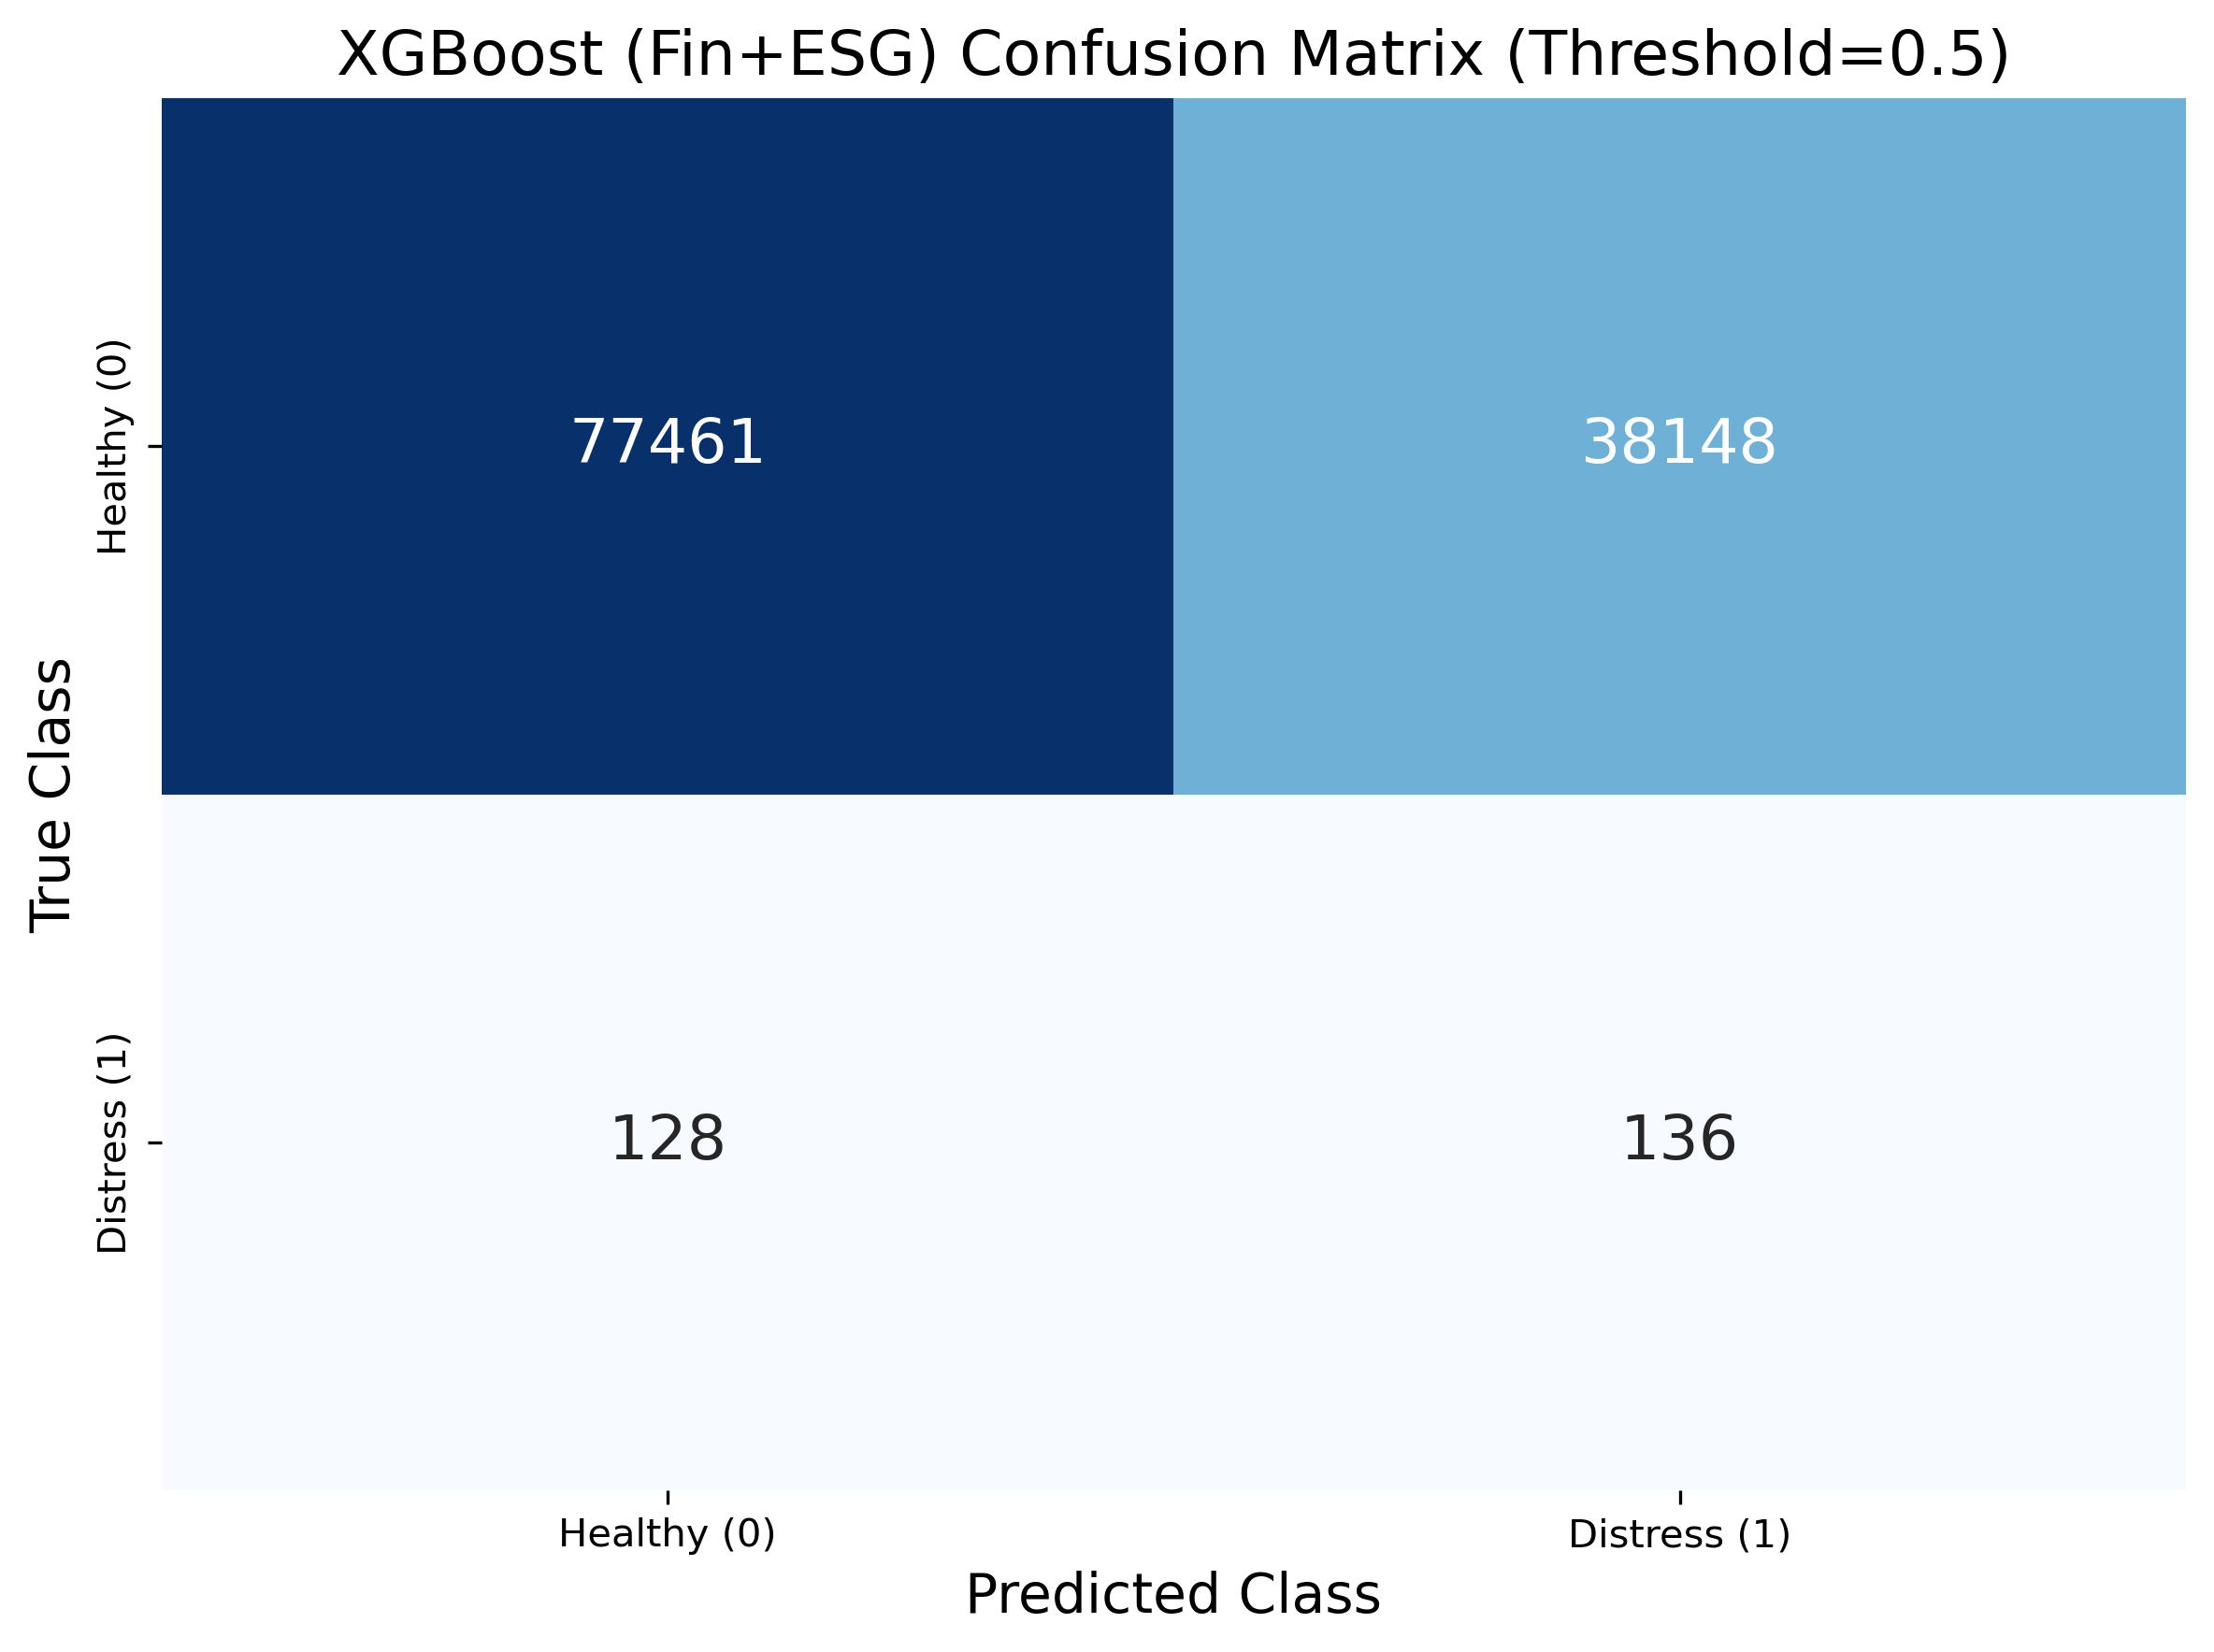
\includegraphics[width=0.86\columnwidth]{reports/figures/confusion_matrix.png}
\caption{Confusion matrix for Model~B at the 0.5 threshold: TN $= 77{,}461$,
FP $= 38{,}148$, FN $= 128$, TP $= 136$. The large false-positive count is a
direct consequence of \code{scale\_pos\_weight} $= 270.75$.}
\label{fig:cm}
\end{figure}

Moving the threshold trades recall against everything else. Two endpoints make
the range concrete. Drop it to 0.30 and the model catches 229 of the 264 events
(86.74\% recall), at 0.2489\% precision and 20.77\% accuracy; that is the regime
you want for an early-warning tool, where a missed collapse costs far more than a
wasted investigation. Push it up to 0.72 and accuracy jumps to 98.20\% while
recall falls to 1.9\%, or 5 events. That second case is the accuracy paradox in a
single line. At 0.2278\% prevalence you can get almost-perfect accuracy just by
calling nearly everything healthy, and end up with a model that is no use for the
job it was built for. The threshold has to be chosen from the relative cost of a
missed event versus a false alarm, not by maximising accuracy.

\subsection{ESG signal diagnostic}
\label{sec:diag}
To see where, if anywhere, the injected ESG signal is lost, we regressed
\code{e\_score} on the relevant distress indicator with a univariate logistic
regression at five points along the pipeline. Table~\ref{tab:diag} has the
coefficients. The estimate stays negative and highly significant ($p < 10^{-12}$)
at every stage. The mild attenuation at Stage~4 ($-0.0336$ versus $-0.0353$) is
the one-year forward shift adding noise to the association, and the larger
standard error at Stage~5 is just the smaller test sample. The recovered numbers
line up with the $-0.0385$ target from Equation~(\ref{eq:coefmap}), with the
residual gap attributable to clipping at the score boundaries and the linear
approximation.

\begin{table}[t]
\caption{Five-stage ESG signal diagnostic: the logistic-regression coefficient
of \code{e\_score}, its standard error, and its $p$-value. Sign and significance
hold at every stage.}
\label{tab:diag}
\centering
\renewcommand{\arraystretch}{1.2}
\begin{tabular}{lccc}
\toprule
Stage & Coef. & SE & $p$-value \\
\midrule
1. Raw panel            & $-0.0353$ & 0.0017 & $3.1 \times 10^{-92}$ \\
2. Post-quality gates   & $-0.0352$ & 0.0017 & $1.5 \times 10^{-90}$ \\
3. Post-feature eng.\   & $-0.0352$ & 0.0017 & $1.5 \times 10^{-90}$ \\
4. Post-forward shift   & $-0.0336$ & 0.0018 & $6.6 \times 10^{-82}$ \\
5. Test set only        & $-0.0364$ & 0.0049 & $1.6 \times 10^{-13}$ \\
\bottomrule
\end{tabular}
\end{table}

\subsection{Attribution}
SHAP puts the three ESG scores at the top of Model~B's global ranking, shown in
Figure~\ref{fig:shap}: \code{g\_score} at mean $|\text{SHAP}| = 0.160$,
\code{e\_score} at 0.145, \code{s\_score} at 0.130. Carbon intensity is much
further down, 19th, at 0.035. The best financial feature,
\code{revenue\_growth\_yoy}, comes in at 0.074, less than half of the weakest of
the top three ESG scores. XGBoost's own gain-based importance tells the same
story. The partial dependence of predicted distress on \code{e\_score}
(Figure~\ref{fig:pdp}) slopes down overall, from roughly 0.45 at the low end to
roughly 0.35 at the high end, about $-0.001$ per unit. It is not perfectly
monotonic; the small wiggles at low \code{e\_score} are what piecewise-constant
tree boundaries do. The overall direction is the one the negative $\gamma$ in the
generator predicts.

\begin{figure}[t]
\centering
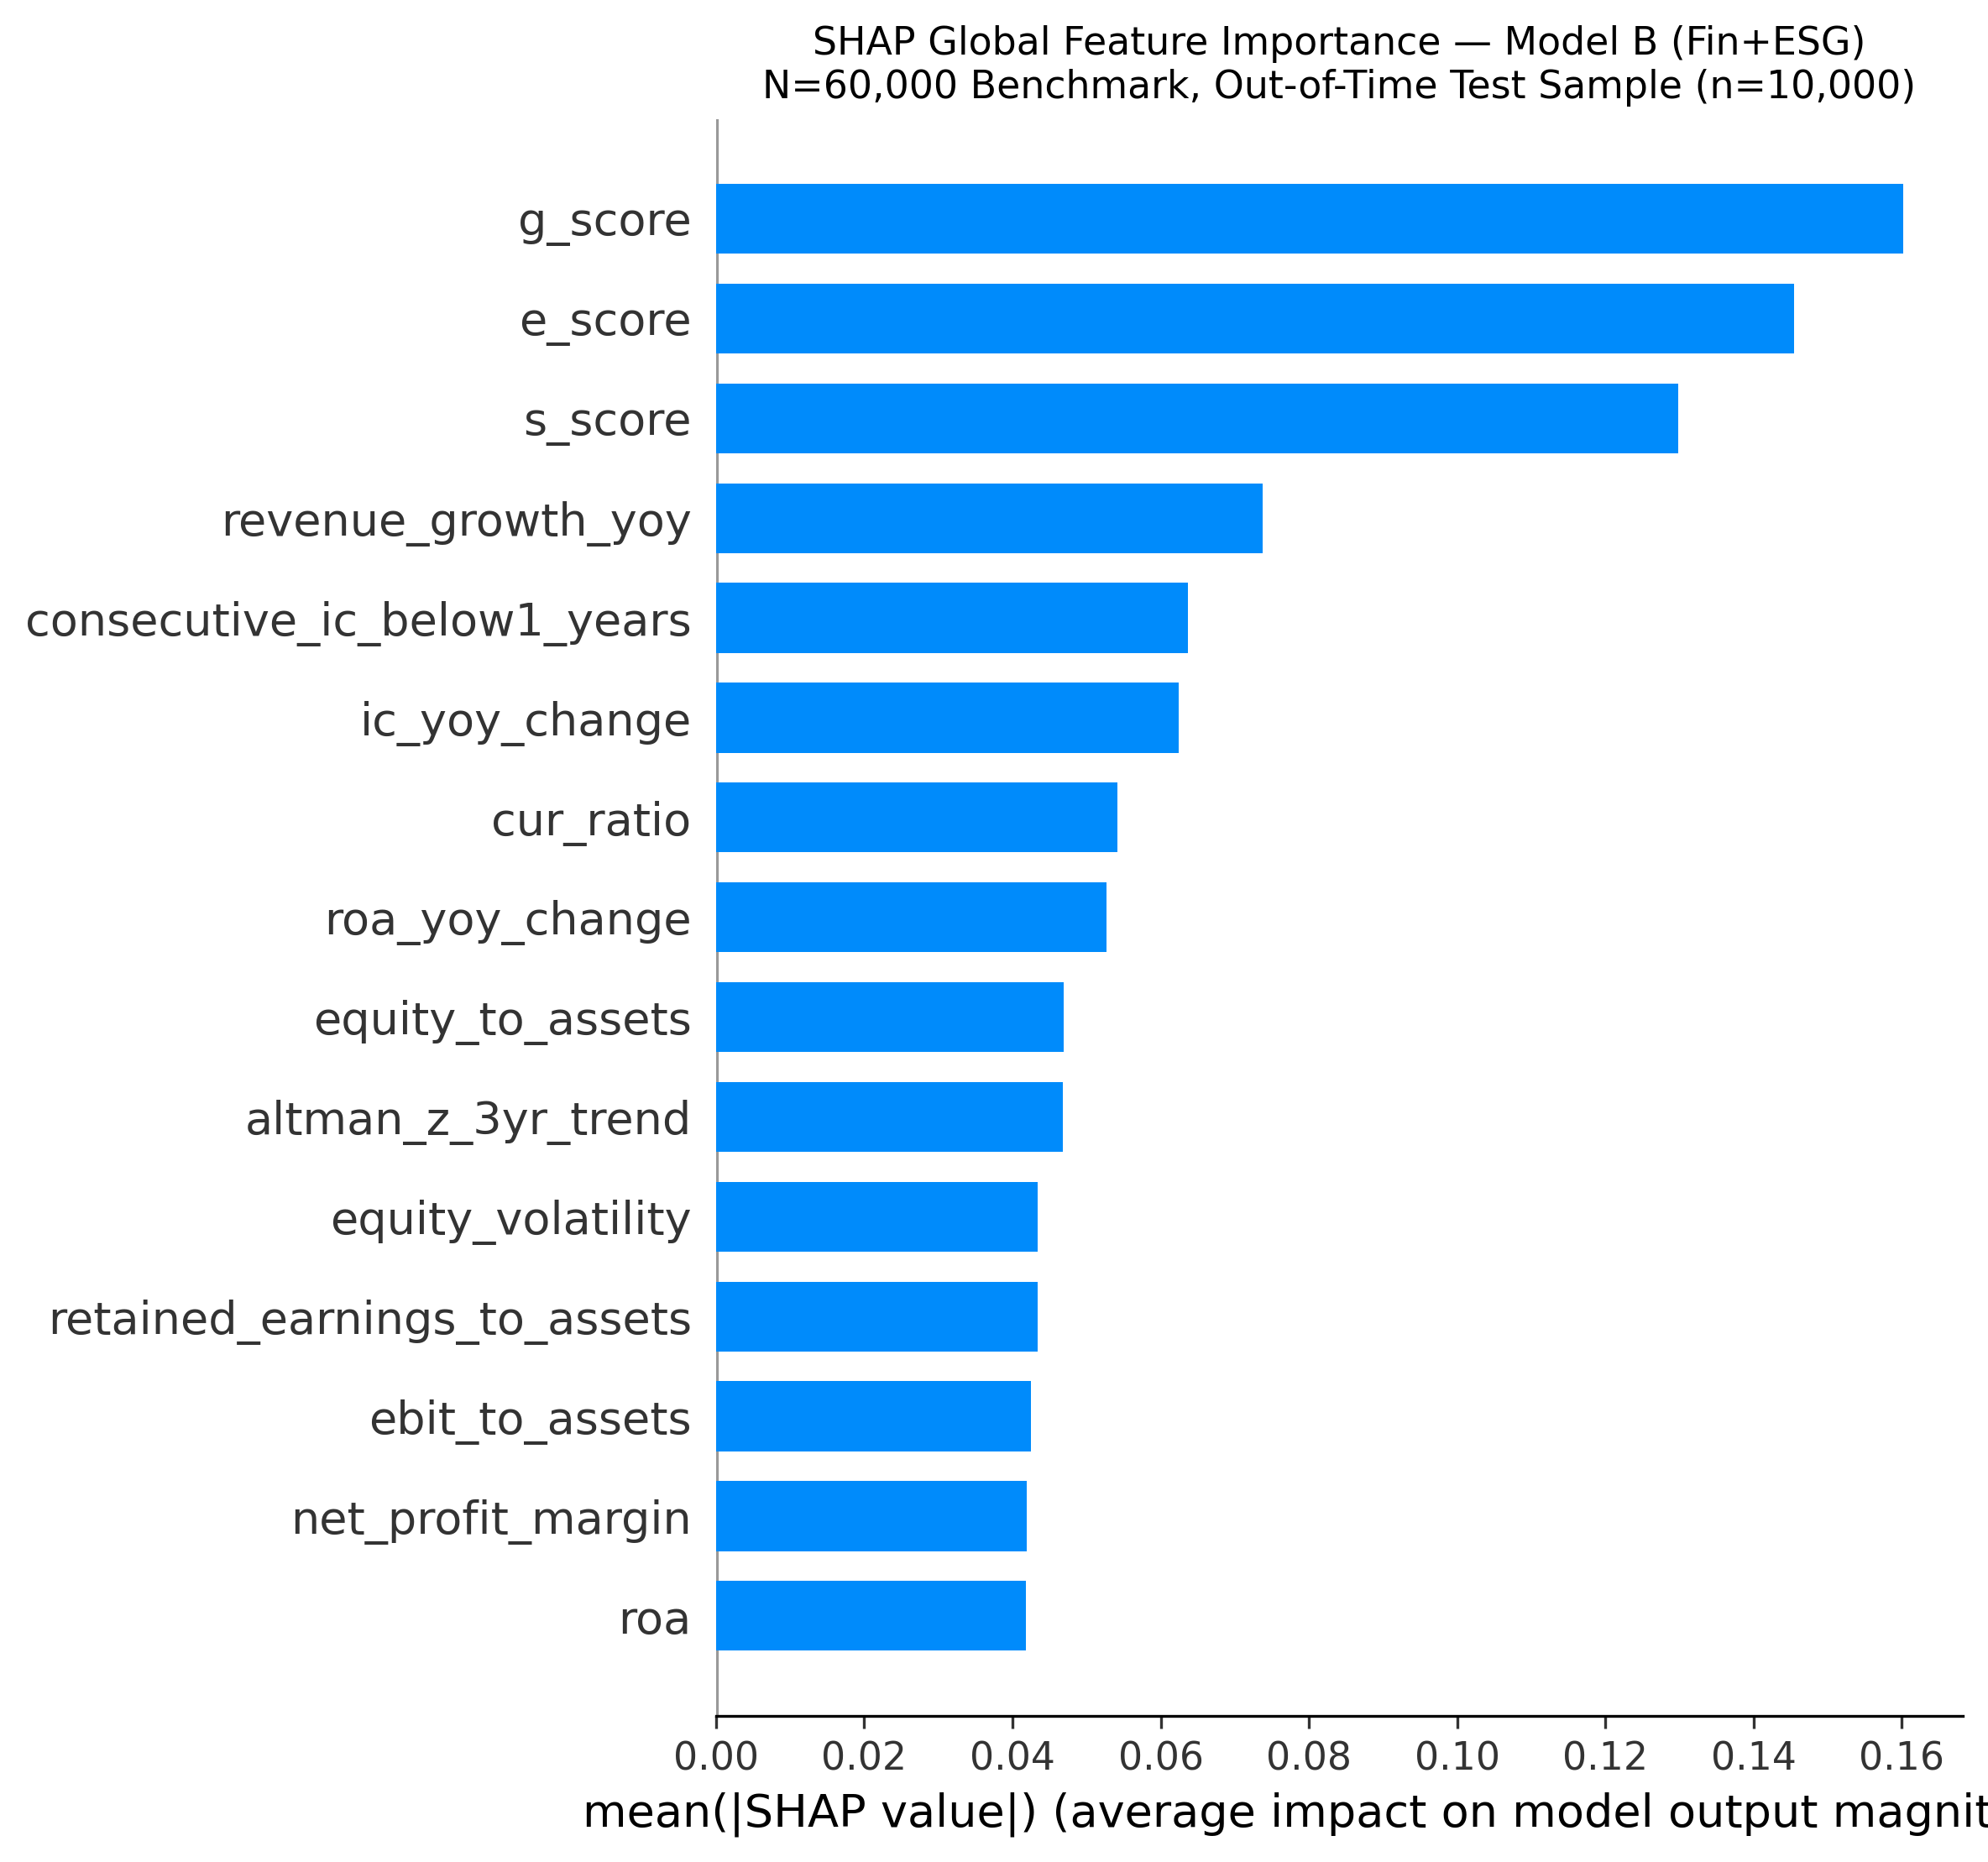
\includegraphics[width=\columnwidth]{reports/figures/shap_summary.png}
\caption{Global SHAP importance for Model~B on 10{,}000 sampled test rows. The
three ESG scores take the top three places by mean $|\text{SHAP}|$; the next
feature, a financial one, is under half the importance of the weakest of the
three.}
\label{fig:shap}
\end{figure}

\begin{figure}[t]
\centering
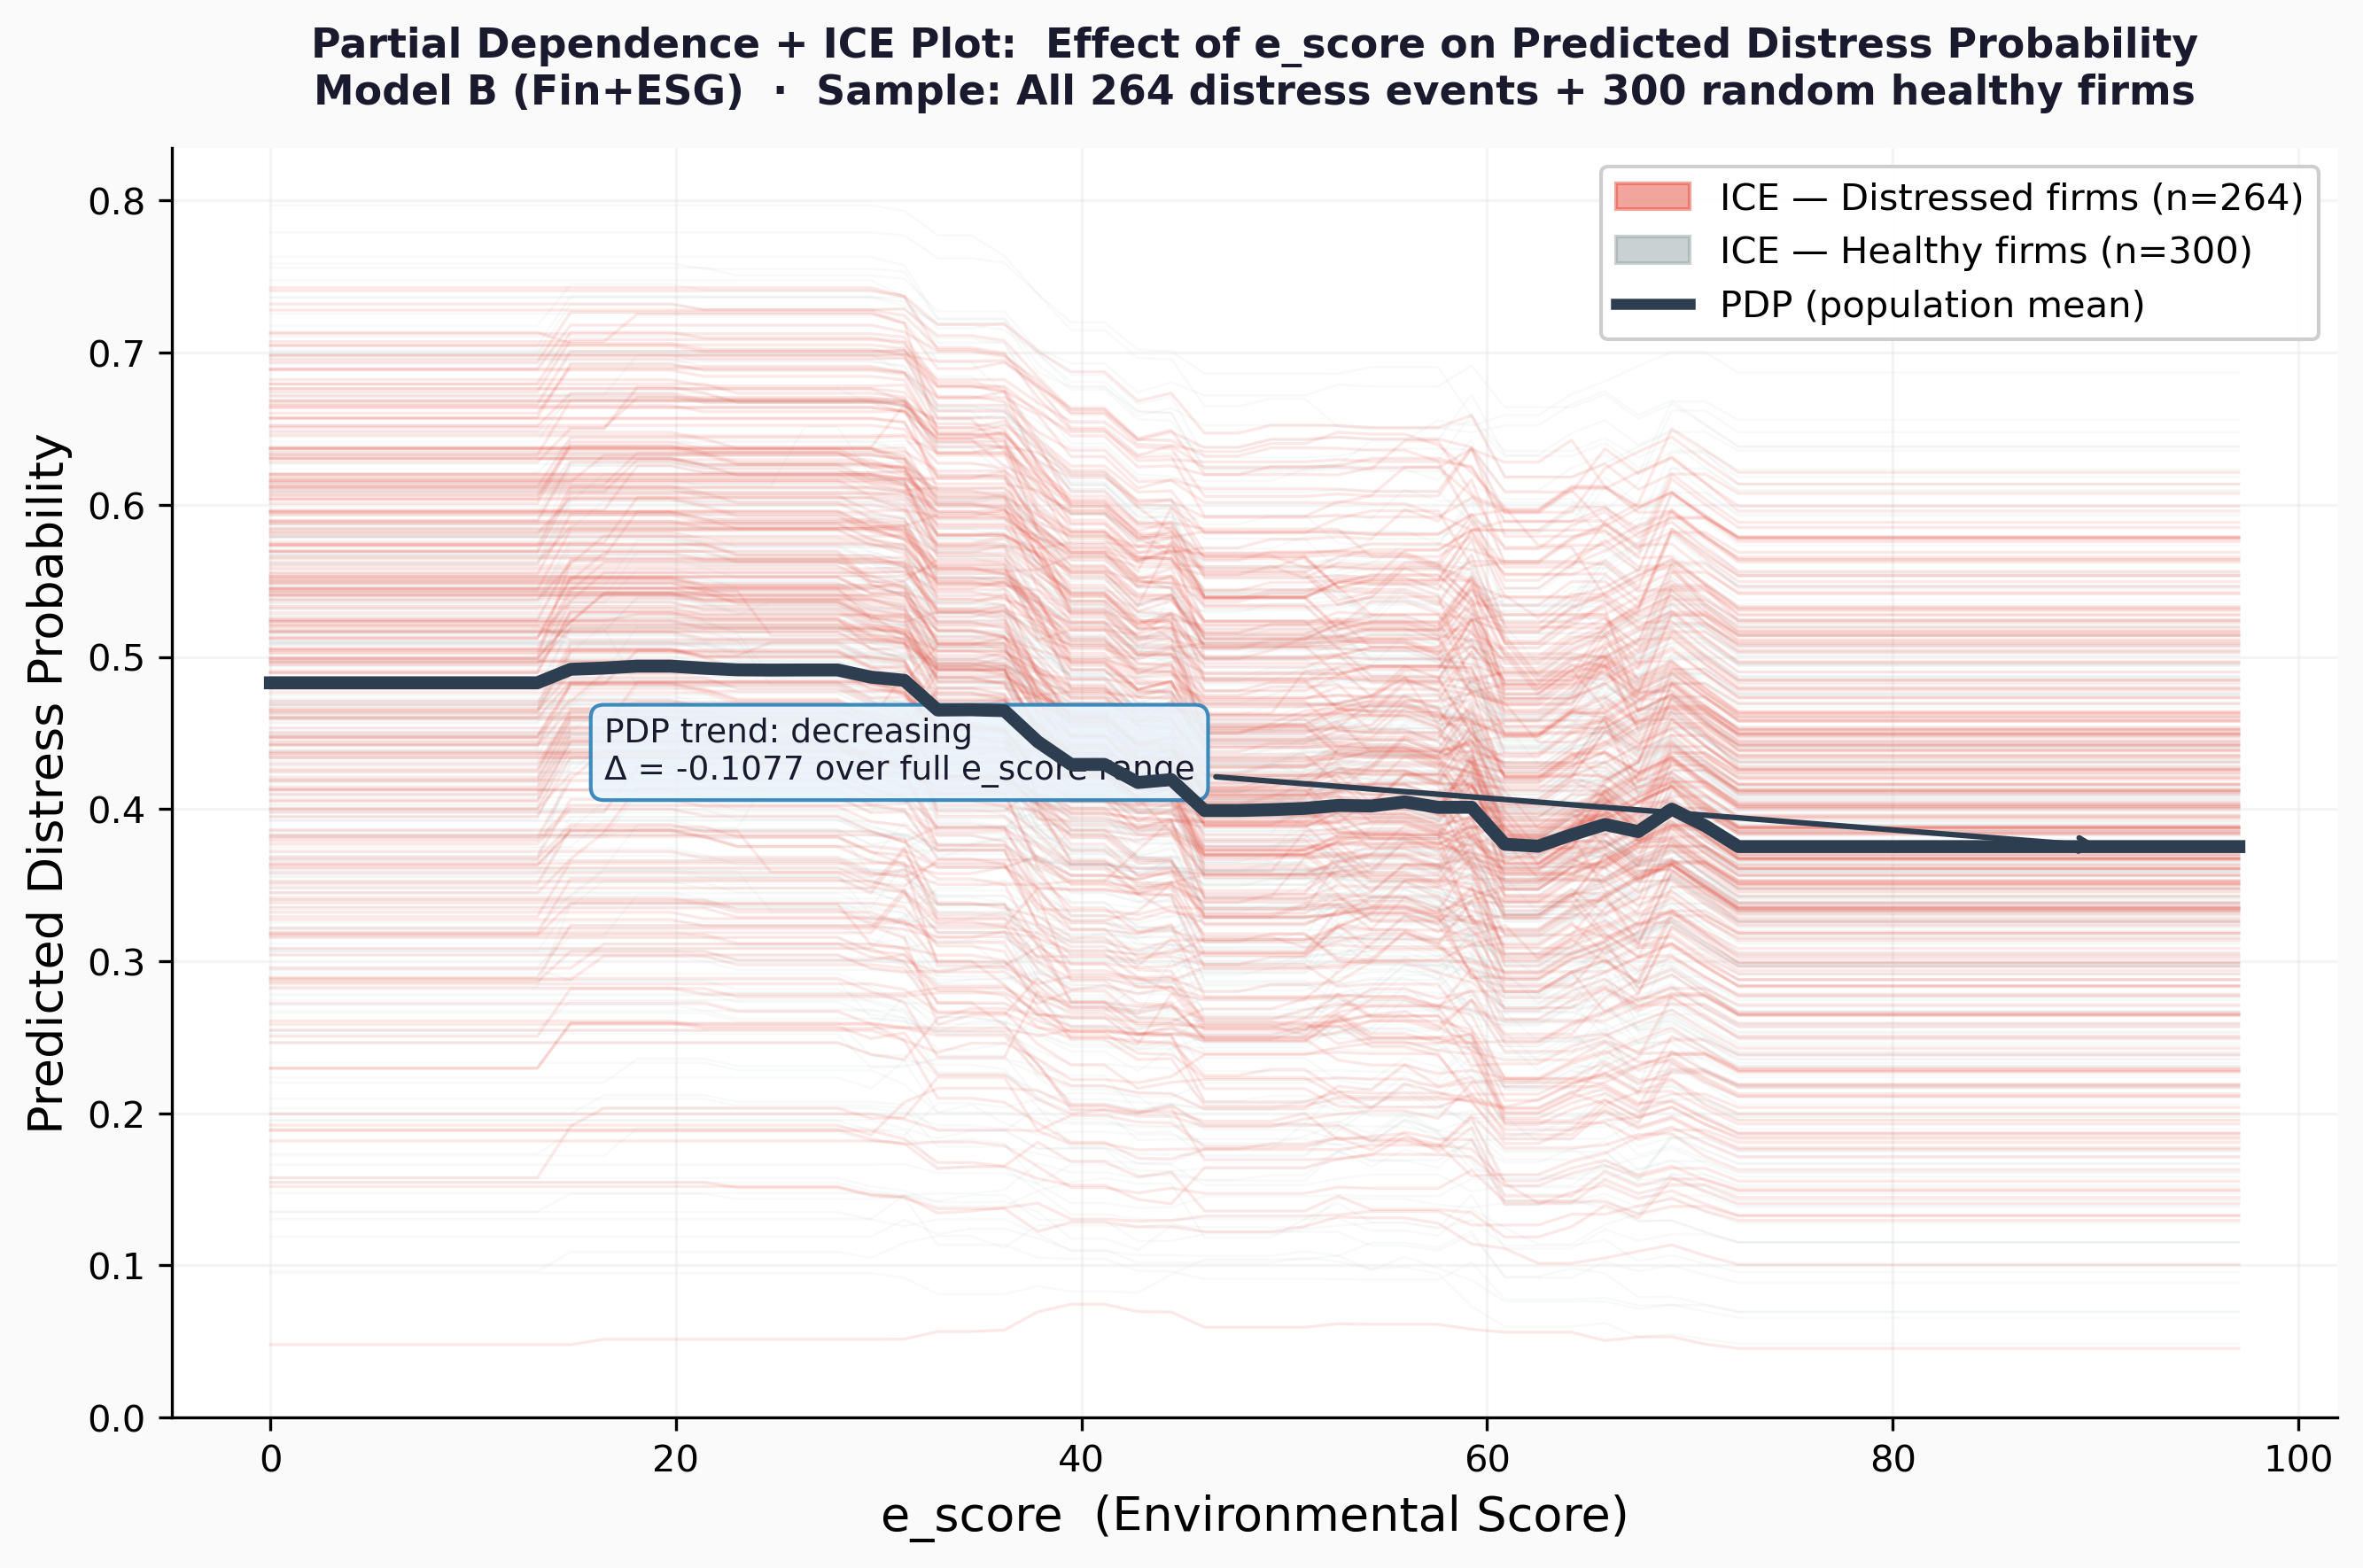
\includegraphics[width=\columnwidth]{reports/figures/pdp_escore.png}
\caption{Partial dependence of Model~B's predicted distress probability on
\code{e\_score}, over 5{,}000 test rows. Predicted distress falls from about 0.45
to about 0.35 across the range, matching the injected protective effect; the
local ripples come from the tree boundaries.}
\label{fig:pdp}
\end{figure}

\section{Discussion}

On RQ1, the number to look at is Model~A's 0.5348. After six circular features
are removed and the one-year gap is enforced, the financial-only model barely
beats chance, and it is nowhere near the 0.95-plus that studies keeping circular
predictors report. Read one way, that difference is a rough estimate of how much
published distress-prediction performance is really the model reconstructing an
accounting identity. Read another way, stripping the circular features is what
clears the room so that any genuine orthogonal signal has somewhere to show up.

RQ2 is where the ESG data earns its place. Model~B recovers the planted signal,
the ROC-AUC gain of $+0.0774$ is significant at the 5\% level, the five-stage
diagnostic shows the coefficient surviving from the raw panel all the way to the
out-of-time test with its sign intact, SHAP ranks the ESG scores one-two-three,
and the partial dependence plot slopes the correct way. Model~B's absolute
ROC-AUC of 0.6117 looks unimpressive next to circular work, and that is by
design. Remove the features that inflate the headline and you are left with an
honest baseline, one you can actually measure an ESG contribution against.

RQ3 is really a warning about how to read Tables~\ref{tab:bench} and
\ref{tab:ablation}. At this prevalence, accuracy and usefulness come apart
completely. Random forest scores 99.58\% and finds nothing; logistic regression
scores 58.56\% and has the best recall in the table. The models with the worse
headline accuracy are the ones doing the job. Any distress model has to be judged
on prevalence-aware metrics, ROC-AUC, PR-AUC, balanced accuracy, positive-class
recall, and accuracy should not be one of them.

The limitations are worth being blunt about. The planted signal, $\gamma = -4.0$,
is a clean, frictionless effect, and real ESG data will almost certainly be
weaker, noisier, and sector-dependent, so none of these synthetic numbers
transfer automatically to real firms. The row-level bootstrap probably
understates the interval width given the paired observations. There was no
hyperparameter search, so the absolute performance levels could move, though the
relative ablation should not. The partial dependence curve is only broadly
monotonic. The 2{,}097 coverage-flagged rows were left in the training set; a
production build might handle them differently. And everything here is tied to
one architecture and one data generator.

For anyone thinking about putting an ESG-augmented credit model into practice,
the practical takeaways are short. Confirm that features circular with the
distress definition are out. Confirm that features and labels are separated in
time. Judge the model on metrics that suit the base rate. And accept that useful
recall in this setting means living with a precision and false-alarm trade-off
that no amount of accuracy tuning will remove. We are not claiming the system is
ready to deploy. What the synthetic study shows is that the pipeline can isolate
an orthogonal signal when one is present.

\section{Conclusion and Future Work}

CRESTA separates features from labels by a year, drops the features that are
circular with the distress definition, and then checks whether a known ESG effect
still comes through. On a synthetic panel of 60{,}000 firms across ten fiscal
years, with a protective ESG signal ($\gamma = -4.0$) built into the generator,
the financial-only model fell to near-chance discrimination (ROC-AUC 0.5348) once
the circular features were removed, and the ESG-augmented model recovered a
significant improvement (ROC-AUC 0.6117; $\Delta$AUC $= +0.0774$, 95\% CI
$[+0.0455,\, +0.1080]$). SHAP put the three ESG variables on top of the global
ranking, and the five-stage diagnostic confirmed the injected coefficient
survived the full pipeline with the right sign and significance.

That establishes controlled signal recovery, and nothing more. It is not
evidence of real-world ESG predictive power and it says nothing about causation.
The obvious next step is to run the same architecture on real Bloomberg
fundamentals joined to India's mandated BRSR disclosures. After that, a
firm-level cluster bootstrap for more conservative inference, a proper
walk-forward hyperparameter search, and a look at other model architectures to
see how far the signal-recovery result carries.

\section*{Reproducibility and Ethics Statement}
Every result here comes from synthetic data generated by the parameters and
equations in Section~III under a fixed seed (42). No real firm data, proprietary
data, or personal information was used. The synthetic panel, the
feature-engineering code, the ablation list, the model configurations, and the
evaluation scripts together are enough to reproduce every number reported. The
framework is a methodological check for research and model validation; its
outputs are not credit ratings, not investment advice, and not a basis for any
automated decision.

\begin{thebibliography}{99}

\bibitem{altman1968}
E.~I. Altman, ``Financial ratios, discriminant analysis and the prediction of
corporate bankruptcy,'' \emph{J. Finance}, vol.~23, no.~4, pp.~589--609, 1968.

\bibitem{ohlson1980}
J.~A. Ohlson, ``Financial ratios and the probabilistic prediction of
bankruptcy,'' \emph{J. Accounting Res.}, vol.~18, no.~1, pp.~109--131, 1980.

\bibitem{merton1974}
R.~C. Merton, ``On the pricing of corporate debt: The risk structure of interest
rates,'' \emph{J. Finance}, vol.~29, no.~2, pp.~449--470, 1974.

\bibitem{jones2015}
S.~Jones, D.~Johnstone, and R.~Wilson, ``An empirical evaluation of the
performance of binary classifiers in the prediction of credit ratings changes,''
\emph{J. Banking Finance}, vol.~56, pp.~72--85, 2015.

\bibitem{sculley2015}
D.~Sculley \emph{et al.}, ``Hidden technical debt in machine learning systems,''
in \emph{Proc. Adv. Neural Inf. Process. Syst. (NeurIPS)}, 2015, pp.~2503--2511.

\bibitem{rabanser2019}
S.~Rabanser, S.~G\"unnemann, and Z.~C. Lipton, ``Failing loudly: An empirical
study of methods for detecting dataset shift,'' in \emph{Proc. Adv. Neural Inf.
Process. Syst. (NeurIPS)}, 2019.

\bibitem{lundberg2017}
S.~M. Lundberg and S.-I. Lee, ``A unified approach to interpreting model
predictions,'' in \emph{Proc. Adv. Neural Inf. Process. Syst. (NeurIPS)}, 2017,
pp.~4765--4774.

\bibitem{chen2016}
T.~Chen and C.~Guestrin, ``XGBoost: A scalable tree boosting system,'' in
\emph{Proc. 22nd ACM SIGKDD Int. Conf. Knowl. Discovery Data Mining}, 2016,
pp.~785--794.

\bibitem{ke2017}
G.~Ke \emph{et al.}, ``LightGBM: A highly efficient gradient boosting decision
tree,'' in \emph{Proc. Adv. Neural Inf. Process. Syst. (NeurIPS)}, 2017,
pp.~3146--3154.

\bibitem{friede2015}
G.~Friede, T.~Busch, and A.~Bassen, ``ESG and financial performance: Aggregated
evidence from more than 2000 empirical studies,'' \emph{J. Sustainable Finance
Investment}, vol.~5, no.~4, pp.~210--233, 2015.

\bibitem{bassen2006}
A.~Bassen and A.~Kovachev, ``ESG-performance and corporate value,'' \emph{SSRN
Electron. J.}, 2006.

\bibitem{lessmann2015}
S.~Lessmann, B.~Baesens, H.-V. Seow, and L.~C. Thomas, ``Benchmarking
state-of-the-art classification algorithms for credit scoring: An update of
research,'' \emph{Eur. J. Oper. Res.}, vol.~247, no.~1, pp.~124--136, 2015.

\bibitem{barboza2017}
F.~Barboza, H.~Kimura, and E.~Altman, ``Machine learning models and bankruptcy
prediction,'' \emph{Expert Syst. Appl.}, vol.~83, pp.~405--417, 2017.

\bibitem{bellotti2009}
A.~Bellotti and J.~Crook, ``Support vector machines for credit scoring and
discovery of significant features,'' \emph{Expert Syst. Appl.}, vol.~36, no.~2,
pp.~3302--3308, 2009.

\end{thebibliography}

\end{document}
